\documentclass[12pt,a4paper]{article} 
\usepackage{graphicx}  % For including images
\usepackage{fancyhdr}  % For headers and footers
\usepackage{geometry}  % For page layout control
\usepackage{tocbibind} % Adds ToC, list of figures to the table of contents
\usepackage{multicol}  % For multiple columns
\usepackage{caption}   % For custom captions
\usepackage{hyperref}  % For clickable ToC
\usepackage{setspace}  % For line spacing
\usepackage{amsmath}
\usepackage{amsfonts}
\usepackage{amssymb}
\usepackage{tcolorbox}
\usepackage{booktabs}
\usepackage{listings}
\usepackage{xcolor}
\usepackage{afterpage} % Avoids blank pages after including large figures

\geometry{margin=1in}
\onehalfspacing  % Set line spacing to 1.5

% Remove section numbering but keep in TOC
\renewcommand{\thesection}{}
\renewcommand{\thesubsection}{}

\lstdefinestyle{customstyle}{
    backgroundcolor=\color{white},
    basicstyle=\ttfamily\footnotesize,
    keywordstyle=\color{blue},
    stringstyle=\color{red},
    commentstyle=\color{green!50!black},
    morekeywords={IF, THEN, ELSE, END, ELSEIF, FIXED, YEAR, SUM, CONTAINS}
}

% Title Page
\title{Business Intelligence Report for Executive Committee\\
\large \textit{\href{https://github.com/JSammut29/ST2187_coursework_2024-25}{Full GitHub Repo - Click Here}}}

\begin{document}

% Title and Executive Summary
\maketitle
\clearpage

\null
\clearpage

\thispagestyle{empty}

\section*{Executive Summary}  % Non-numbered section for the executive summary

This report provides a comprehensive analysis of the company’s order data since 2020, focusing on uncovering commercially significant insights to drive decision-making. 

In 2023, the company achieved a profit of \$504,411; from 8,572 orders generating total sales revenue of \$4,300,785.

The United States and APAC continue to dominate order volumes, with California, New York, Texas, Australia, China, and India being top-performing regions. \textbf{Office Supplies}, particularly \textbf{Binders} and \textbf{Storage}, drive the highest order volumes, although \textbf{Binders} exhibit troubling margin variability. Meanwhile, \textbf{Tables} have been identified as a loss leader, playing a pivotal role as customers who purchase tables contribute significantly to overall profitability.

Over the last four years, margins have remained stable, averaging \textbf{11\%} and capped at \textbf{50\%}, indicating strong operational control but limited room for further margin growth. \textbf{Paper sales} emerged as the most consistent and profitable.

The company's \textbf{order priority system} shows no correlation with profitability or retention rates, suggesting a need for re-evaluation. \textbf{Customer retention} remains strong, with a \textbf{120\% retention rate} among top clients, but \textbf{new customer acquisition} is declining, necessitating refined marketing efforts.

Projected profits for 2024 and 2025 are \textbf{\$585,000} and \textbf{\$685,000}, respectively, with opportunities to exceed these forecasts through targeted optimization of product margins, customer acquisition strategies, and order prioritization improvements. The report offers actionable recommendations aimed at enhancing profitability and ensuring sustainable growth.

\newpage

\null
\clearpage

\tableofcontents  % Generates the Table of Contents automatically

% Temporarily set margins to zero for this page
\newgeometry{margin=0cm}

% Full Page PDF Image
\noindent
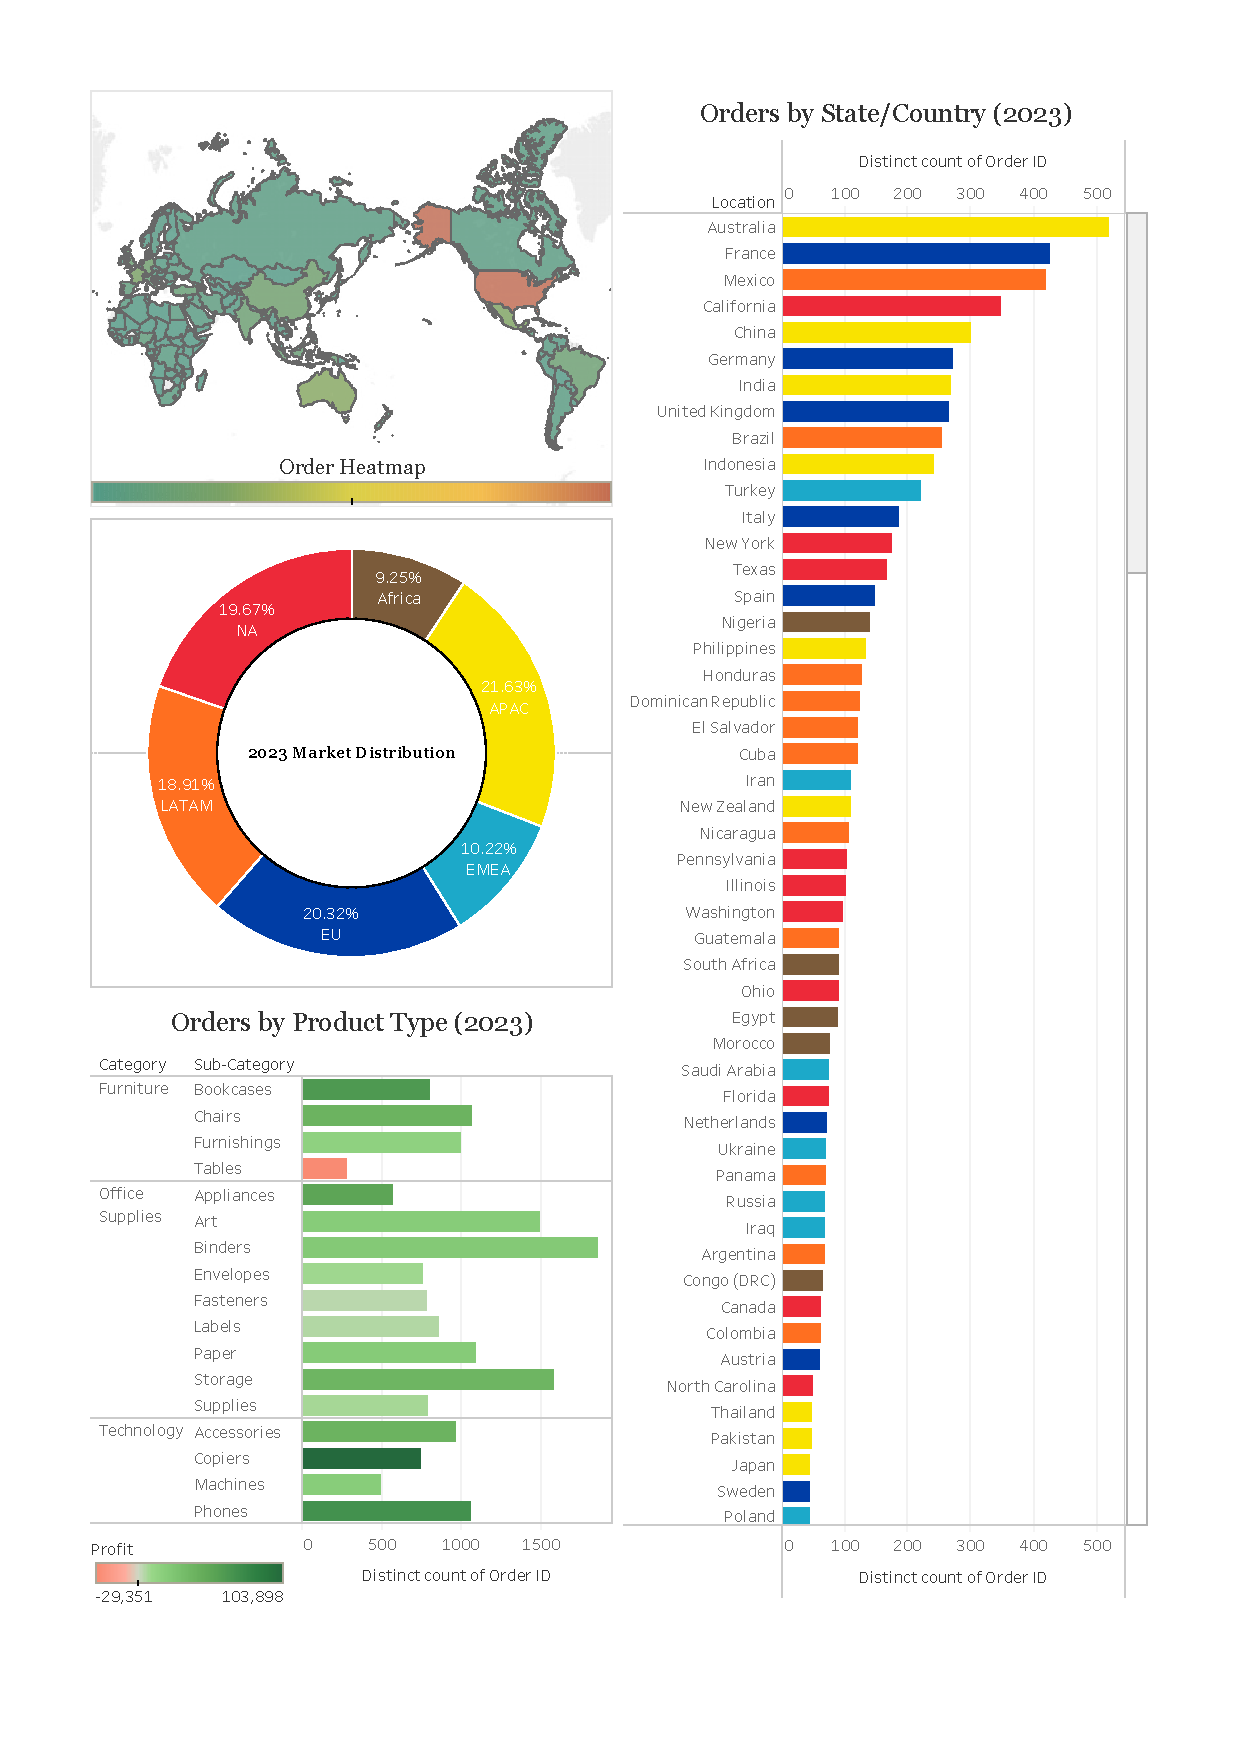
\includegraphics[width=\paperwidth,height=\paperheight,keepaspectratio]{Dashboard1.pdf}

% Restore original margins
\restoregeometry

\newpage

% Dashboard Section for Dashboard 1
\section{Dashboard 1: Geographic and Product Distribution}

In 2023, the distribution of clients remained largely stable, with broad growth across all regions. \textbf{The United States continues to dominate} in terms of order volume, driven by strong contributions from states like \textbf{California, New York, and Texas}, accounting for a combined total of \textbf{1,694 orders}. The \textbf{Asia Pacific (APAC)} market also maintained its position as a key player, primarily fuelled by demand from \textbf{Australia, China, and India}.

In terms of products, \textbf{Office Supplies} continue to be the core driver of orders, with \textbf{Binders} being the most frequently ordered item. Following closely are \textbf{Storage, Art, and Paper}, with \textbf{Storage} emerging as the highest profit generator among office supplies. However, not all products performed equally well, with \textbf{Tables} standing out as the slowest-selling and a known \textbf{loss generator}. Despite this, tables play a strategic role, as discussed later in the analysis.

% Temporarily set margins to zero for this page
\newgeometry{margin=0cm}
\vspace*{-0.5cm} % Adjust vertical space if necessary

% Full Page PDF Image
\noindent
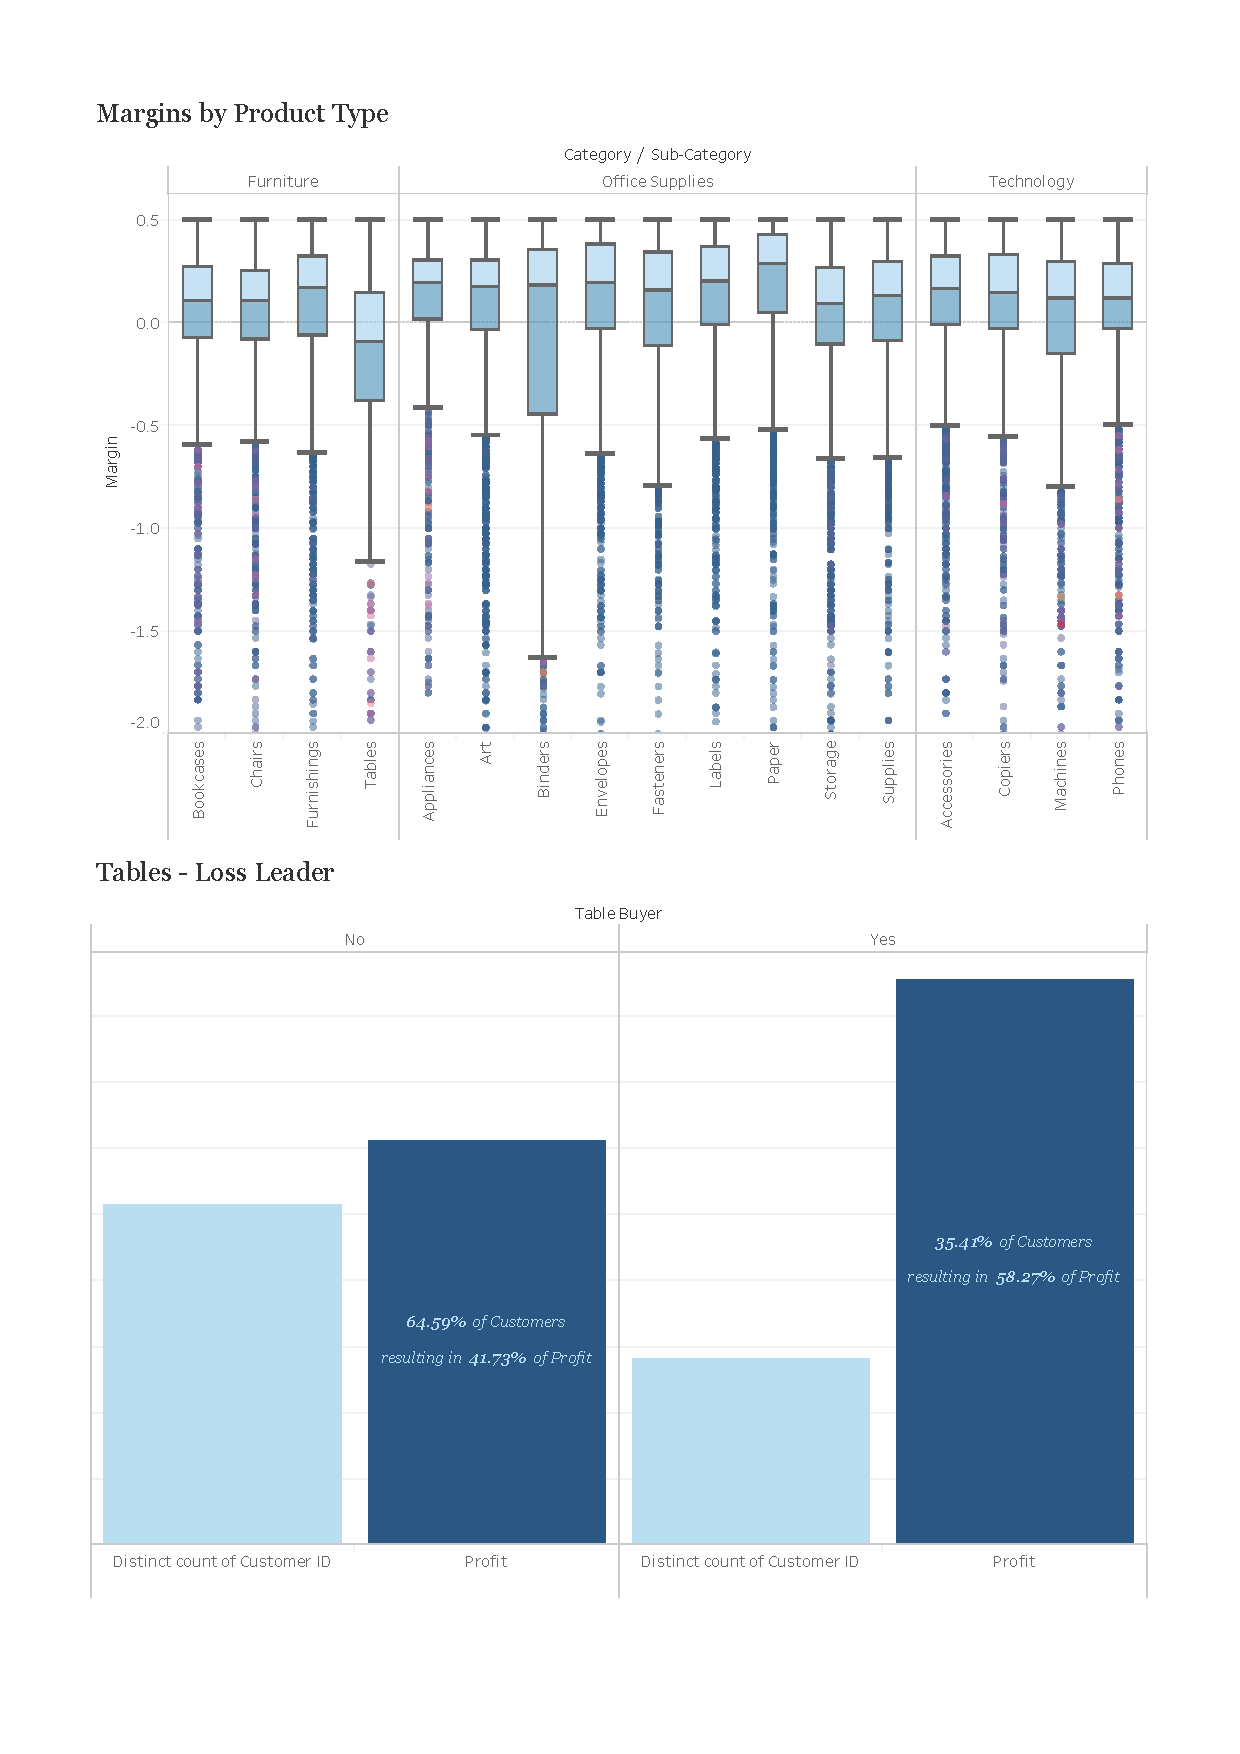
\includegraphics[width=\paperwidth,height=\paperheight,keepaspectratio]{Dashboard2.pdf}

% Restore original margins
\restoregeometry

\newpage

% Dashboard Section for Dashboard 2
\section{Dashboard 2: Margins and Profitability}

Over each of the last four years, \textbf{margins have averaged 11\%, with a cap at 50\%}. This consistency reflects strong operational control, but also suggests that there’s limited room for significant margin improvement at the overall company level. However, individual product lines show varying performances, highlighting areas for strategic focus.

\textbf{Paper sales} continue to demonstrate strong and reliable margins, with a median rate of \textbf{28\%}. Given the combination of high order volume and consistent margins, paper is a key product that should be further leveraged to enhance overall profitability. Efforts to increase paper sales will undoubtedly strengthen our bottom line.

In contrast, \textbf{Binders}, despite being our most frequently ordered product, have a concerning margin spread. The median margin is \textbf{18\%}, but the \textbf{25th percentile} reveals a margin as low as \textbf{negative 45\%}. This inconsistency suggests potential inefficiencies in pricing or fulfilment. Addressing these disparities could unlock further profit potential in this product category.

Meanwhile, \textbf{Tables} are confirmed as loss leaders, as they play an important strategic role. Customers who purchase tables make up only \textbf{35\%} of our customer base, yet they contribute \textbf{58\%} of total profits. This outsized profitability justifies continuing to absorb losses on table sales, but we should remain vigilant for any reversal of this trend. Monitoring customer behaviour around table purchases and identifying opportunities for upselling could further capitalize on this dynamic.

% Temporarily set margins to zero for this page
\newgeometry{margin=0cm}
\vspace*{-0.5cm} % Adjust vertical space if necessary

% Full Page PDF Image
\noindent
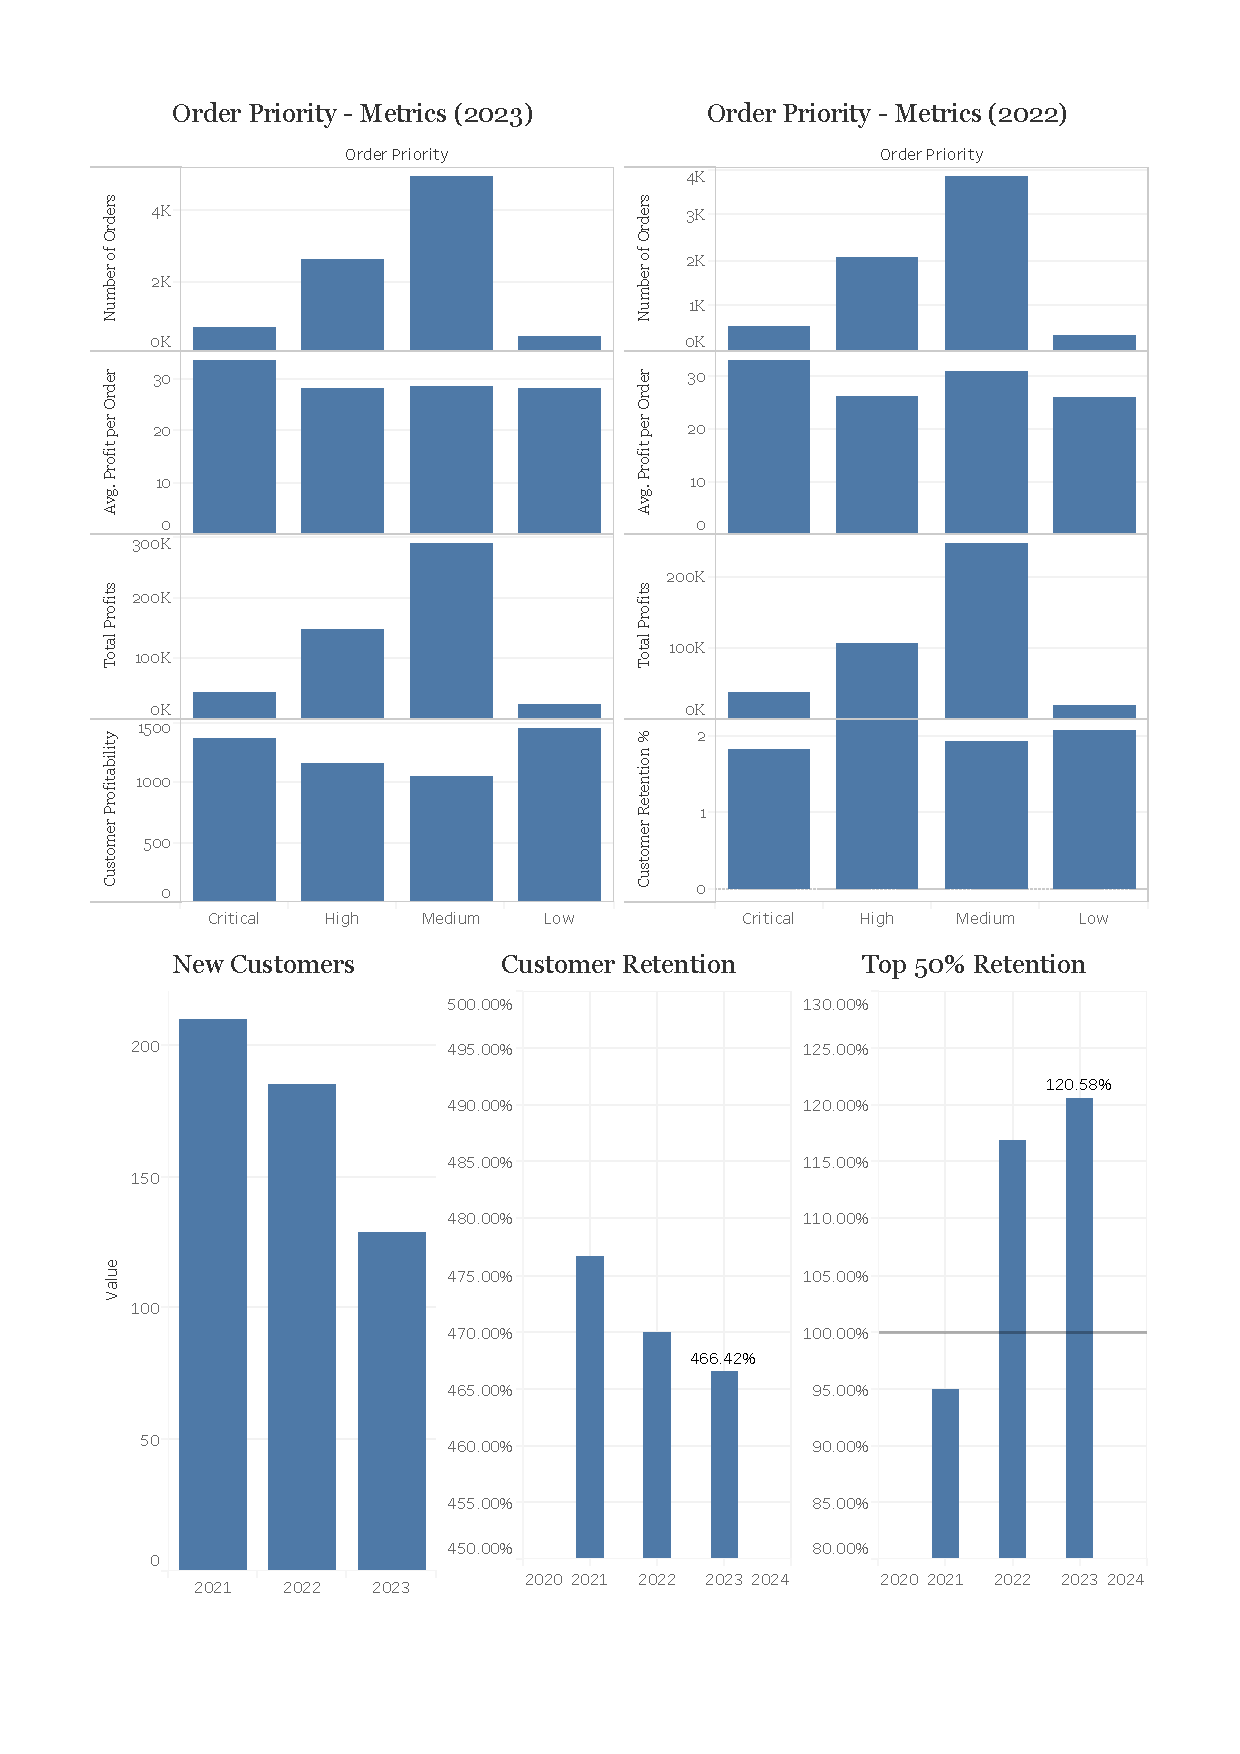
\includegraphics[width=\paperwidth,height=\paperheight,keepaspectratio]{Dashboard3.pdf}

% Restore original margins
\restoregeometry

\newpage

% Dashboard Section for Dashboard 3
\section{Dashboard 3: Order Priority and Customer Retention}

Our analysis of \textbf{Order Priority Assignment} reveals an opportunity for improvement. Currently, there is no clear alignment between \textbf{high-priority orders} and \textbf{higher profitability} or \textbf{better retention rates}. This lack of correlation suggests that our order prioritization process may not be adequately benefiting the most profitable clients or orders. A thorough evaluation is necessary to determine whether high-priority orders are receiving superior service. If they are, we should ensure that our most profitable clients and orders are prioritized. If not, we might consider eliminating the system and focusing on streamlining our overall processes.

Despite this, \textbf{customer retention remains robust}, with an average retention rate still above \textbf{450\%}. Additionally, for our top 50\% of clients by revenue, retention has grown to \textbf{120\%} in 2023, up from 116\% last year. This indicates growing loyalty amongst high-revenue customers, which is essential for sustaining long-term profitability. However, \textbf{new customer acquisition} has been trending downward year-over-year. In 2023, we gained \textbf{129 new customers}, resulting in a net growth of our customer base by \textbf{57 clients}; which is lower than the previous two years having achieved 82 net new clients last year and 63 net new clients the year before. While strong retention helps stabilize the business, the decline in new customers could slow overall growth. Investment in targeted marketing campaigns or promotional offers for new customers could reverse this trend, improving the balance between retention and acquisition.

% Temporarily set margins to zero for this page
\newgeometry{margin=0cm}
\vspace*{-0.5cm} % Adjust vertical space if necessary

% Full Page PDF Image
\noindent
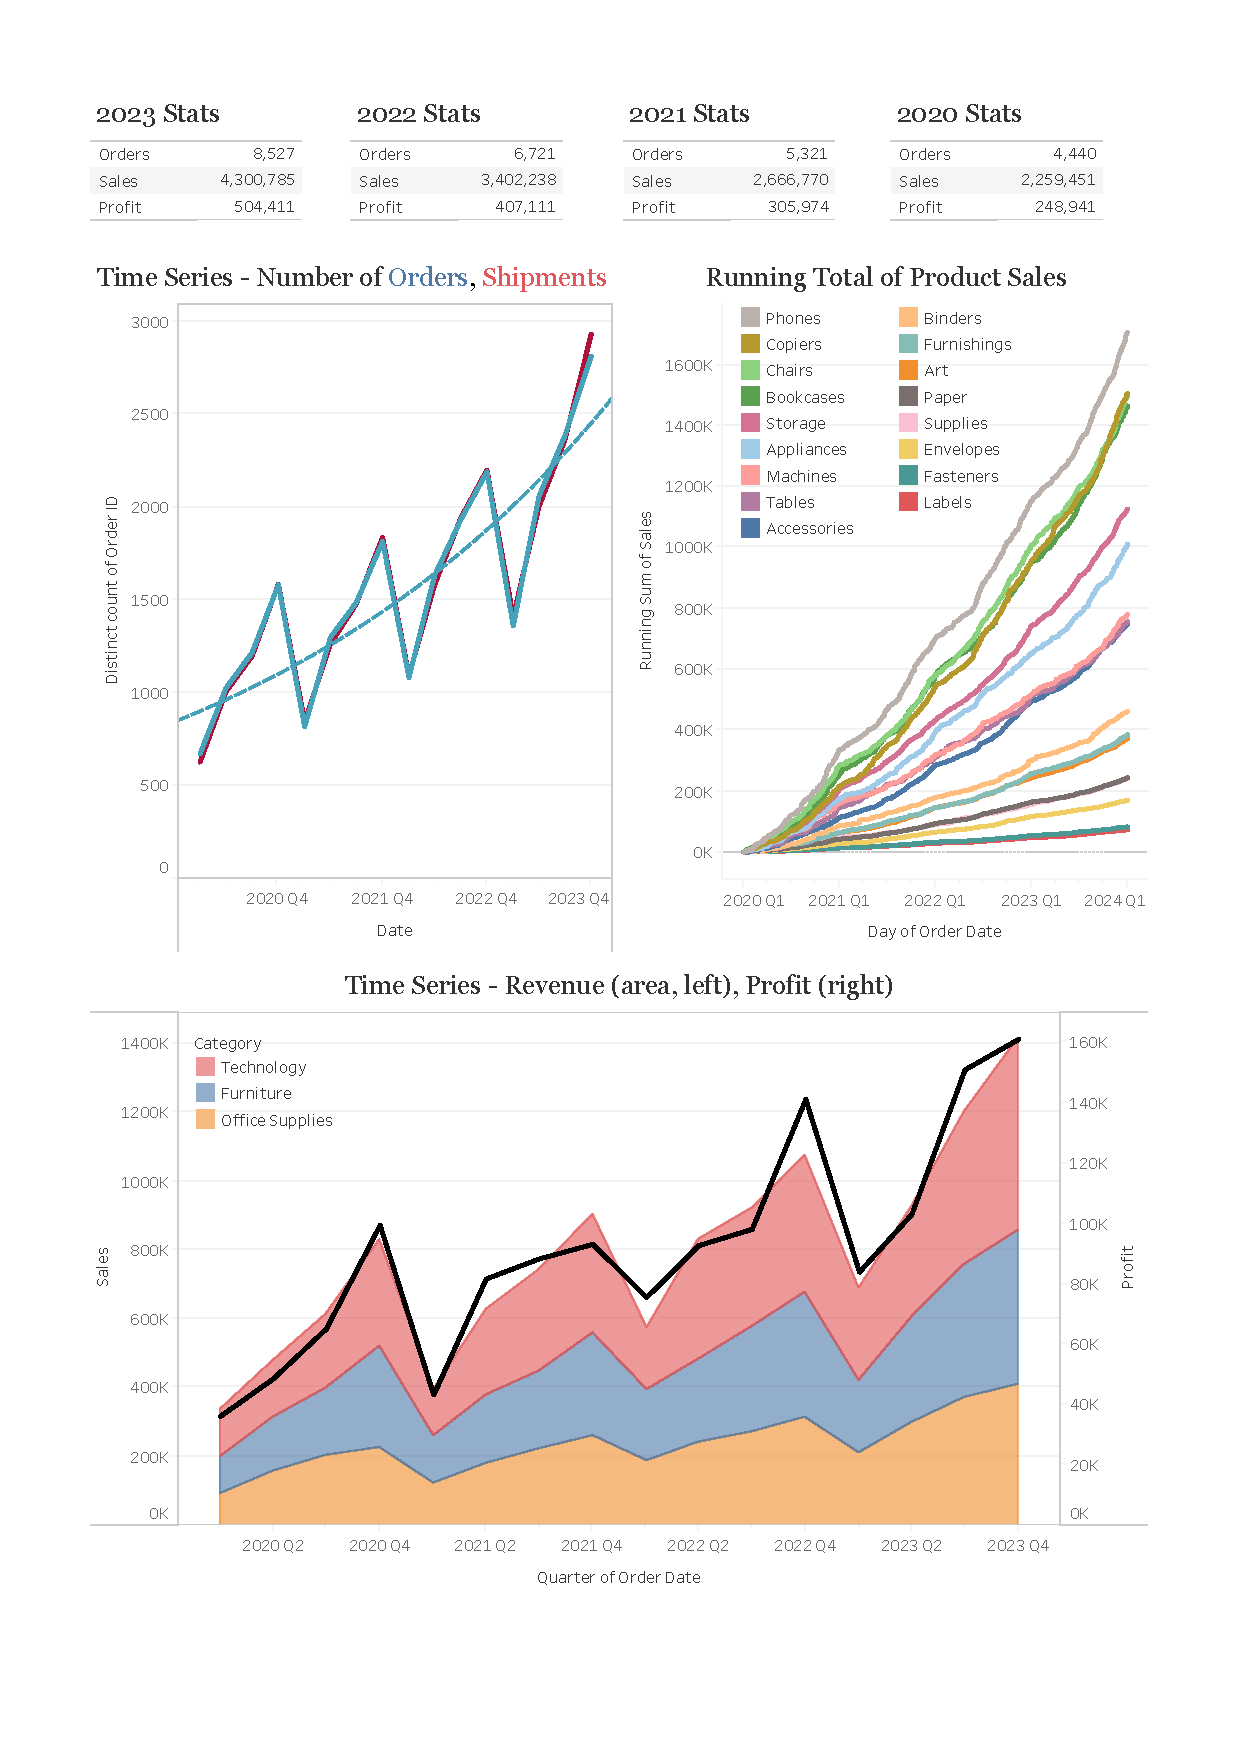
\includegraphics[width=\paperwidth,height=\paperheight,keepaspectratio]{Dashboard4.pdf}

% Restore original margins
\restoregeometry

\newpage

% Dashboard Section for Dashboard 4
\section{Dashboard 4: Year-over-Year Growth}

\textbf{Profit for 2023} reached just over \textbf{\$500,000} from just over \$400,000 last year, representing a \textbf{24\% year-over-year increase} from 2022. This aligns with the trend of increasing order counts and revenues seen over the past few years. The revenue was almost evenly split between the \textbf{Technology, Furniture, and Office Supplies} categories, demonstrating broad-based growth across product lines. 

We also continue to observe \textbf{seasonality} in order volumes, with slower starts to the year followed by sustained growth through the remaining quarters. Understanding this seasonality will be essential for optimizing inventory management and staffing in the future.

% Temporarily set margins to zero for this page
\newgeometry{margin=0cm}
\vspace*{-0.5cm} % Adjust vertical space if necessary

% Full Page PDF Image
\noindent
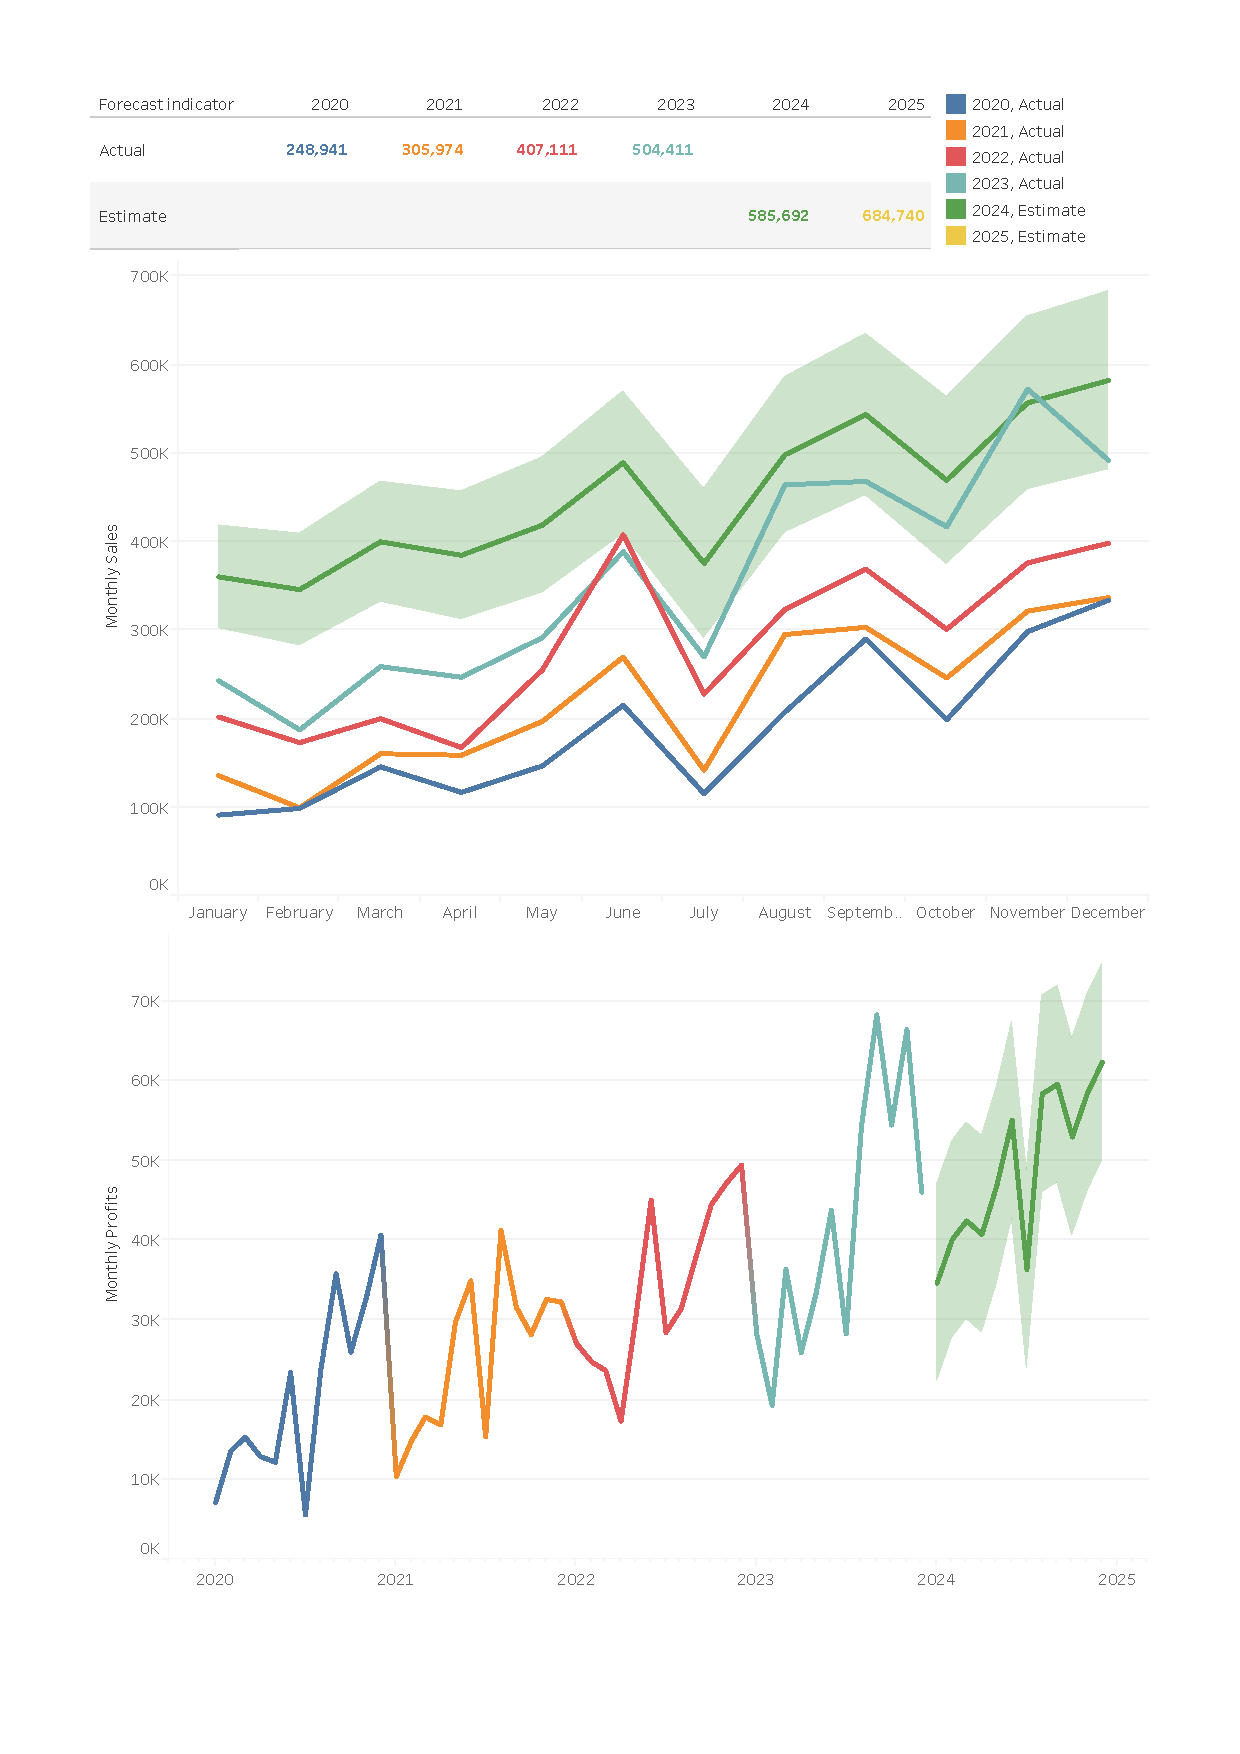
\includegraphics[width=\paperwidth,height=\paperheight,keepaspectratio]{Dashboard6.pdf}

% Restore original margins
\restoregeometry

\newpage

% Dashboard Section for Dashboard 5
\section{Dashboard 5: Forecasting Future Performance}

Looking ahead, our analysis of \textbf{source data} from January 2020 to December 2023 projects \textbf{steady profit growth} through 2025. Based on current trajectories, we expect profits to reach \textbf{\$585,000 in 2024} and \textbf{\$685,000 in 2025}. However, these projections are based on historical trends, and we anticipate that implementing the optimizations discussed today could help us exceed these estimates.

By addressing margin inconsistencies in key products like binders and strategically continuing to support loss leaders like tables, we can improve overall profitability. Additionally, refining our approach to order prioritization and investing in new customer acquisition will ensure that we maintain strong growth in both revenue and profit over the next two years.

\newpage

\section*{Word Count}
Total word count: 838 words

\vspace*{2cm}

\begin{tcolorbox}[colback=white!10!white, colframe=blue!75!black, title= Loss Leader, sharp corners=southwest, enhanced]
A loss leader is a pricing tactic in which a product is offered at a price lower than its production cost to entice customers to purchase additional items. The main objective is to boost overall sales volume and gain market share by attracting customers to the store or platform. This strategy can result in increased profits on complementary products or services.
\end{tcolorbox}

\vspace*{2cm}

\section{Technical Appendix: Calculated Fields}

\vspace*{1cm}

\textbf{Location}
\begin{lstlisting}[style=customstyle]
IF [Country] = 'United States' THEN [State] ELSE [Country] END
\end{lstlisting}
\vspace*{1cm}

\textbf{New for 2021}
\begin{lstlisting}[style=customstyle]
IF [Total Sales 2020] = 0 AND [Total Sales 2021] > 0 THEN
[Customer ID] ELSE "0" END
\end{lstlisting}
\vspace*{1cm}

\textbf{New for 2022}
\begin{lstlisting}[style=customstyle]
IF [Total Sales 2021] = 0 AND [Total Sales 2022] > 0 THEN
[Customer ID] ELSE "0" END
\end{lstlisting}
\vspace*{1cm}

\textbf{New for 2023}
\begin{lstlisting}[style=customstyle]
IF [Total Sales 2022] = 0 AND [Total Sales 2023] > 0 THEN
[Customer ID] ELSE "0" END
\end{lstlisting}
\vspace*{1cm}

\textbf{Standardised Market}
\begin{lstlisting}[style=customstyle]
IF [Country] = 'Austria' THEN 'EU'
ELSEIF [Country] = 'Mongolia' THEN 'EMEA'
ELSEIF [Market] = 'US' OR [Market] = 'Canada' THEN 'NA'
ELSE [Market] END
\end{lstlisting}
\vspace*{1cm}

\textbf{Margin}
\begin{lstlisting}[style=customstyle]
[Profit]/[Sales]
\end{lstlisting}
\vspace*{1cm}

\textbf{Order Year}
\begin{lstlisting}[style=customstyle]
YEAR([Order Date])
\end{lstlisting}
\vspace*{1cm}

\textbf{Placeholder}
\begin{lstlisting}[style=customstyle]
0.1
\end{lstlisting}
\vspace*{1cm}

\textbf{Retention \%}
\begin{lstlisting}[style=customstyle]
IF [Order Year] = 2021 AND [New for 2021] = "0" THEN
[Sales for Year] / [Sales last Year]
ELSEIF [Order Year] = 2022 AND [New for 2022] = "0" THEN
[Sales for Year] / [Sales last Year]
ELSEIF [Order Year] = 2023 AND [New for 2023] = "0" THEN
[Sales for Year] / [Sales last Year]
ELSE NULL END
\end{lstlisting}
\vspace*{1cm}

\textbf{Retention \% (forward)}
\begin{lstlisting}[style=customstyle]
[Sales next Year] / [Sales for Year]
\end{lstlisting}
\vspace*{1cm}

\textbf{Retention \% (forward) (top 50\%)}
\begin{lstlisting}[style=customstyle]
IF [Sales for Year] > 1500 THEN
[Sales next Year] / [Sales for Year]
ELSE NULL END
\end{lstlisting}
\vspace*{1cm}

\textbf{Sales for Year}
\begin{lstlisting}[style=customstyle]
{FIXED [Customer ID], YEAR([Order Date]): SUM([Sales])}
\end{lstlisting}
\vspace*{1cm}

\textbf{Sales if 2020}
\begin{lstlisting}[style=customstyle]
IF YEAR([Order Date]) = 2020 THEN [Sales]
ELSE 0 END
\end{lstlisting}
\vspace*{1cm}

\textbf{Sales if 2021}
\begin{lstlisting}[style=customstyle]
IF YEAR([Order Date]) = 2021 THEN [Sales]
ELSE 0 END
\end{lstlisting}
\vspace*{1cm}

\textbf{Sales if 2022}
\begin{lstlisting}[style=customstyle]
IF YEAR([Order Date]) = 2022 THEN [Sales]
ELSE 0 END
\end{lstlisting}
\vspace*{1cm}

\textbf{Sales if 2023}
\begin{lstlisting}[style=customstyle]
IF YEAR([Order Date]) = 2023 THEN [Sales]
ELSE 0 END
\end{lstlisting}
\vspace*{1cm}

\textbf{Sales last Year}
\begin{lstlisting}[style=customstyle]
IF [Order Year] = 2020 THEN NULL
ELSEIF [Order Year] = 2021 THEN
IF [New for 2021] = "0" THEN [Total Sales 2020]
ELSE NULL END
ELSEIF [Order Year] = 2022 THEN
IF [New for 2022] = "0" THEN [Total Sales 2021]
ELSE NULL END
ELSEIF [Order Year] = 2023 THEN
IF [New for 2023] = "0" THEN [Total Sales 2022]
ELSE NULL END END
\end{lstlisting}
\vspace*{1cm}

\textbf{Sales next Year}
\begin{lstlisting}[style=customstyle]
IF [Order Year] = 2023 THEN NULL
ELSEIF [Order Year] = 2022 THEN [Total Sales 2023]
ELSEIF [Order Year] = 2021 THEN [Total Sales 2022]
ELSEIF [Order Year] = 2020 THEN [Total Sales 2021]
END
\end{lstlisting}
\vspace*{1cm}

\textbf{Table Buyer}
\begin{lstlisting}[style=customstyle]
{FIXED [Customer ID]: MAX([Table Order])}
\end{lstlisting}
\vspace*{1cm}

\textbf{Table Order}
\begin{lstlisting}[style=customstyle]
IF CONTAINS([Sub-Category], 'Table') THEN 1 ELSE 0 END
\end{lstlisting}
\vspace*{1cm}

\textbf{Total Profitability}
\begin{lstlisting}[style=customstyle]
{FIXED [Customer ID]: SUM([Profit])}
\end{lstlisting}
\vspace*{1cm}

\textbf{Total Sales 2020}
\begin{lstlisting}[style=customstyle]
{FIXED [Customer ID]: SUM([Sales if 2020])}
\end{lstlisting}
\vspace*{1cm}

\textbf{Total Sales 2021}
\begin{lstlisting}[style=customstyle]
{FIXED [Customer ID]: SUM([Sales if 2021])}
\end{lstlisting}
\vspace*{1cm}

\textbf{Total Sales 2022}
\begin{lstlisting}[style=customstyle]
{FIXED [Customer ID]: SUM([Sales if 2022])}
\end{lstlisting}
\vspace*{1cm}

\textbf{Total Sales 2023}
\begin{lstlisting}[style=customstyle]
{FIXED [Customer ID]: SUM([Sales if 2023])}
\end{lstlisting}
\vspace*{1cm}

\end{document}
